\documentclass[border=0mm]{standalone}
\usepackage{pgfplots}
\usepgfplotslibrary{groupplots}
\pgfplotsset{compat=1.17}
\usepackage{xcolor}
\usepackage{xstring}
\usepackage{tikz}



\definecolor{color1}{rgb}{0,0.4470,0.7410}
\definecolor{color2}{rgb}{0.8500,0.3250,0.0980}
\definecolor{color3}{rgb}{0.9290,0.6940,0.1250}
\definecolor{color4}{rgb}{0.4940,0.1840,0.5560}
\definecolor{color5}{rgb}{0.4660,0.6740,0.1880}


\begin{document}

\pgfplotsset{
compat=1.11,
legend image code/.code={
\draw[mark repeat=2,mark phase=2]
plot coordinates {
(0cm,0cm)
(0.3cm,0cm)        %% default is (0.3cm,0cm)
(0.6cm,0cm)         %% default is (0.6cm,0cm)
};%
}%
}%


\pgfdeclarelayer{background layer}%
\pgfdeclarelayer{foreground layer}%
\pgfsetlayers{background layer,main,foreground layer}%

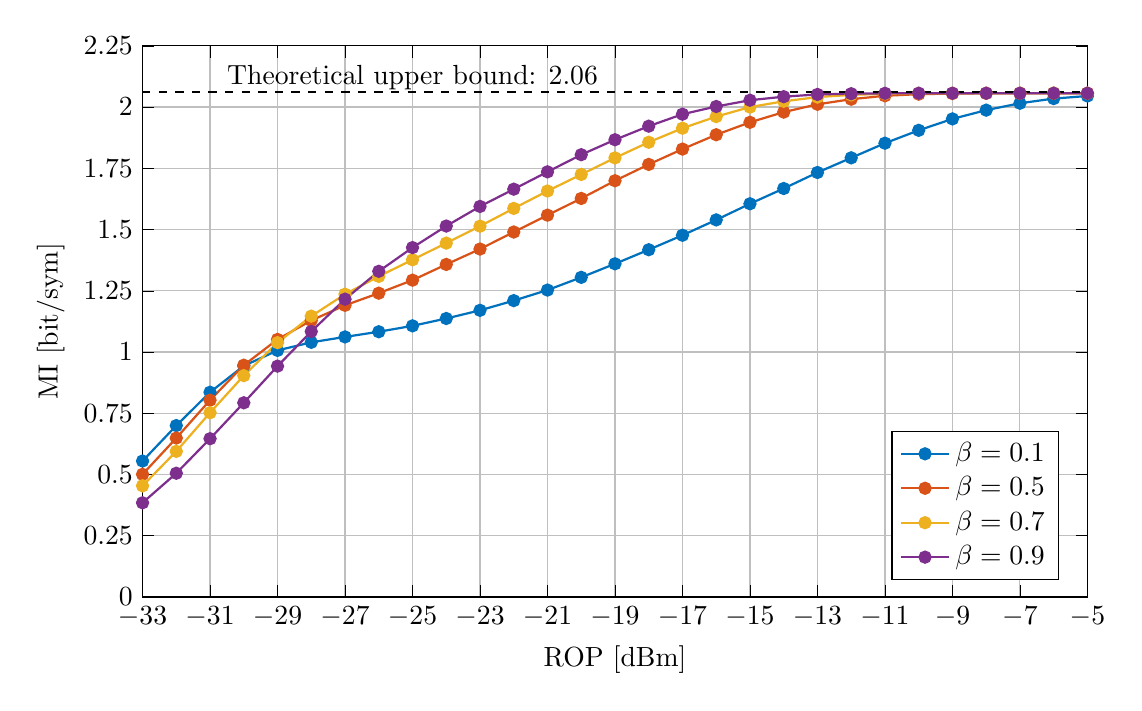
\begin{tikzpicture}[
]
\begin{axis}[%
width=12cm,
height=7cm,
scale only axis,
every outer x axis line/.append style={black},
every x tick label/.append style={font=\color{black}},
every x tick/.append style={black},
xmin=-33,
xmax=-5,
xlabel={ROP [dBm]},
every outer y axis line/.append style={black},
every y tick label/.append style={font=\color{black}},
every y tick/.append style={black},
ymin=0,
ymax=2.25,
ylabel={MI [bit/sym]},
axis background/.style={fill=white},
xmajorgrids,
ymajorgrids,
xtick={-33,-31,...,-5},
ytick={0,0.25,...,2.25},
legend pos=south east
]
\addplot [thick,color1, mark=*] coordinates {(-33,0.5550601896622804)(-32,0.6997469757513218)(-31,0.8357846590937884)(-30,0.9434913596869245)(-29,1.0065550209268117)(-28,1.0396153099441214)(-27,1.0616826650847602)(-26,1.0828115031523626)(-25,1.1068715476225246)(-24,1.1368143280050353)(-23,1.1701764578160432)(-22,1.2098127873878282)(-21,1.2529456175754408)(-20,1.3048817357451368)(-19,1.3601915748567803)(-18,1.4175736482086967)(-17,1.4766144680255404)(-16,1.5394010799355378)(-15,1.6052308710254006)(-14,1.6674996269385514)(-13,1.7329080961418502)(-12,1.7927158409863482)(-11,1.8524386050470631)(-10,1.9050156782976966)(-9,1.951665392031474)(-8,1.9873722747160814)(-7,2.015485886972068)(-6,2.034525961683681)(-5,2.0451669083356605)};
\addlegendentry{$\beta=0.1$}

\addplot [thick,color2, mark=*] coordinates {(-33,0.5007123838728993)(-32,0.6488327015237294)(-31,0.8033629939172853)(-30,0.9461395558394793)(-29,1.0515196656053678)(-28,1.128901509643629)(-27,1.190594233338826)(-26,1.2402671742951978)(-25,1.2933446121711953)(-24,1.3575502112444655)(-23,1.4203824130278633)(-22,1.4898546059981026)(-21,1.5586856413446022)(-20,1.62696215038157)(-19,1.699235052023628)(-18,1.7658399521631025)(-17,1.8284150329716518)(-16,1.8869849285738318)(-15,1.9376688343173232)(-14,1.9793256465171265)(-13,2.0112235394287015)(-12,2.0320279083552744)(-11,2.0460632239135967)(-10,2.052505402818985)(-9,2.05500265252367)(-8,2.056181879567641)(-7,2.0563663865613226)(-6,2.0564852897235864)(-5,2.0564852897235864)};
\addlegendentry{$\beta=0.5$}

\addplot [thick,color3, mark=*] coordinates {(-33,0.45395756010490357)(-32,0.5945180318115111)(-31,0.7523009666784928)(-30,0.903614807256388)(-29,1.0382737254092376)(-28,1.1463962811353285)(-27,1.2360071562141608)(-26,1.3087743050693927)(-25,1.3766969804284923)(-24,1.4446334102256175)(-23,1.5137895473660192)(-22,1.5862286362591063)(-21,1.6572614960175613)(-20,1.7248775820881492)(-19,1.7925548383641552)(-18,1.856291795887211)(-17,1.9136140939631787)(-16,1.9610407650067199)(-15,1.999867897511639)(-14,2.0234780714883445)(-13,2.0407077277143473)(-12,2.0497004438655013)(-11,2.054124732406011)(-10,2.0559568860077384)(-9,2.056326645698643)(-8,2.0564456657492625)(-7,2.0564457212848777)(-6,2.0564852897235864)(-5,2.0564852897235864)};
\addlegendentry{$\beta=0.7$}

\addplot [thick,color4, mark=*] coordinates {(-33,0.3845936891962943)(-32,0.5051730954058593)(-31,0.6461519101843566)(-30,0.7927601724897343)(-29,0.94240594450127)(-28,1.0837847626924393)(-27,1.2158124768807386)(-26,1.3293921924014738)(-25,1.426316897189949)(-24,1.5143090301369362)(-23,1.5942970215852632)(-22,1.6647535056162102)(-21,1.7355094696418645)(-20,1.8055036895756444)(-19,1.8665865362394192)(-18,1.9219605316363273)(-17,1.970797474221098)(-16,2.002304630811233)(-15,2.027879955847506)(-14,2.0423248332886956)(-13,2.051541942689265)(-12,2.054436098607258)(-11,2.0561024755443533)(-10,2.056445607437049)(-9,2.0564852897235864)(-8,2.0564852897235864)(-7,2.0564852897235864)(-6,2.0564852897235864)(-5,2.0564852897235864)};
\addlegendentry{$\beta=0.9$}

\addplot [thick,black, dashed] coordinates{(-34,2.06)(-4,2.06)};
\coordinate (xd) at (axis cs: -31,2.12);


\end{axis}
\node [anchor=west,inner sep=6] at (xd) {Theoretical upper bound: 2.06};

\end{tikzpicture}


\end{document}
























